%----------------------------------------------------------------------------------------
%	PACKAGES AND OTHER DOCUMENT CONFIGURATIONS
%----------------------------------------------------------------------------------------

\documentclass{resume_new} % Use the custom resume.cls style

\usepackage{array}
\usepackage{hyperref}
\usepackage{tikz}

\usepackage{fontspec}
\usepackage{fontawesome}

\hypersetup{
    colorlinks=true,
    urlcolor=blue,
}

\begin{document}
\begin{paracol}{2}
%----------------------------------------------------------------------------------------
%
%   FIRST COLUMN
%
%----------------------------------------------------------------------------------------

%----------------------------------------------------------------------------------------
%	Title Section
%----------------------------------------------------------------------------------------
\hfill{\MakeUppercase{\huge\bf Ian Gallagher}}\hfill

%----------------------------------------------------------------------------------------
%	Education
%----------------------------------------------------------------------------------------

\section*{Education}
\hrule
{\bf Cal Poly, San Luis Obispo} \hfill Grad. June 2021 \\
B.S. \textbf{Mathematics} \hfill GPA \textbf{3.9} \\
Minor \textbf{Computer Science}
%----------------------------------------------------------------------------------------
%	WORK EXPERIENCE SECTION
%----------------------------------------------------------------------------------------

\section*{Experience}
\hrule

\begin{resumeList}{Software Team Member}{November 2019 - Present}{Cal Poly CubeSat Laboratory}{}
\item Software Lead for NASA ER-2 payload designed to record plane's in-flight vibrational profile and interface with CPCL XCube payload carrier.
\item Designed for Linux platforms. Programming in C and Python.
\end{resumeList}

\begin{resumeList}{Frost Research Scholar}{June 2019 - September 2019}{Cal Poly Mathematics Department}{}
\item Researched the underlying mathematical properties of low order glacial climate models.
\item Investigated the interactions between internal free oscillations and external forcing signals, focusing on changes in model behavior over a range of parameter regimes.
\item Model and analysis code written in Matlab.
\end{resumeList}

\begin{resumeList}{Frost Research Scholar}{June 2020 - September 2020}{Cal Poly Mathematics Department}{}
\item Part of a team of three undergraduate students investigating the structure of the maximal tori of the generalized quaternions.
\item Work was primarily focused on the moduli spaces of maximal commutative sub-algebras. 
\item Used and developed tools in non-commutative ring theory, category theory, and other related fields.
\end{resumeList}

\switchcolumn % paracol command to toggle column
%----------------------------------------------------------------------------------------
%
%   Second Column
%
%----------------------------------------------------------------------------------------

%----------------------------------------------------------------------------------------
%   Contact Information
%----------------------------------------------------------------------------------------
\section*{Contact Me}
\hrule

\begin{tabular}{ @{} >{\bfseries}l @{\hspace{6ex}} l }
    \faPhone            & (831)\,818-9080 \\
    \faEnvelope         & iangallagherm@gmail.com \\
    \faGlobe            & 6249 Gushee Street \\
                        & Felton, CA \\
    \faLinkedinSquare   & \href{https://www.linkedin.com/in/ianmichaelgallagher}{ianmichaelgallagher} \\
    \faGithubSquare     & \href{https://www.github.com/in/iangallagherm}{iangallagherm}
\end{tabular}

%----------------------------------------------------------------------------------------
%   Skills 
%----------------------------------------------------------------------------------------

\section*{Awards}
\hrule

\begin{resumeList}{Outstanding Junior Award}{June 2020}{Cal Poly Mathematics Department}{}
\item Awarded to a single student in the math major for demonstrating superior leadership skills and the ability to work effectively with peers and faculty.
\end{resumeList}

\begin{resumeList}{Van Duyne Scholarship}{June 2019, 2020}{Cal Poly Mathematics Department}{}
\item Two time recipient of scholarship intended for high-achieving students in the mathematics major.
\end{resumeList}
%----------------------------------------------------------------------------------------
%   Awards
%----------------------------------------------------------------------------------------

\section*{Technical Skills}
\hrule

%\begin{tabular}{ @{} >{\bfseries}l @{\hspace{6ex}} l }
%Programming Languages \ & Python, Java, C, Matlab \\
%Software \& Tools & Linux, Bash, Git, Valgrind, GDB, Latex  \\
%\end{tabular}
{\bf Programming Languages} \\
Python, Java, C, Matlab \\
{\bf Software Tools} \\
Linux, Bash, Git, Valgrind, GDB, Latex


\begin{tikzpicture}
\node [anchor=west] at (-3,0.3) {Java};
\draw [fill=lightgray] (0,0) rectangle (5,.5);
\draw [fill={rgb:red,1;green,2;blue,3}] (0,0) rectangle (3,.5);
\end{tikzpicture}

\vspace{.05cm}
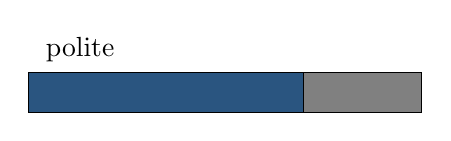
\begin{tikzpicture}
\node [anchor=west] at (.1,.8) {polite};
\draw [fill=gray] (0,0) rectangle (5,.5);
\draw [fill={rgb:red,1;green,2;blue,3}] (0,0) rectangle (3.5,.5);
\end{tikzpicture}

\vspace{.05cm}
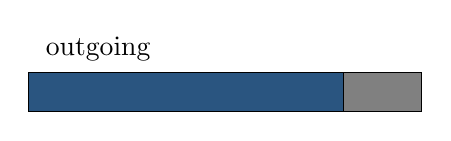
\begin{tikzpicture}
\node [anchor=west] at (.1,.8) {outgoing};
\draw [fill=gray] (0,0) rectangle (5,.5);
\draw [fill={rgb:red,1;green,2;blue,3}] (0,0) rectangle (4,.5);
\end{tikzpicture}

\vspace{.05cm}
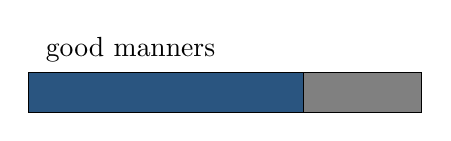
\begin{tikzpicture}
\node [anchor=west] at (.1,.8) {good manners};
\draw [fill=gray] (0,0) rectangle (5,.5);
\draw [fill={rgb:red,1;green,2;blue,3}] (0,0) rectangle (3.5,.5);
\end{tikzpicture}

\vspace{.05cm}
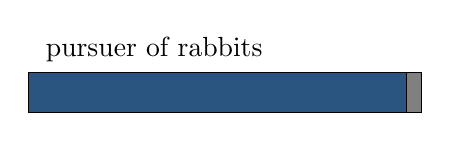
\begin{tikzpicture}
\node [anchor=west] at (.1,.8) {pursuer of rabbits};
\draw [fill=gray] (0,0) rectangle (5,.5);
\draw [fill={rgb:red,1;green,2;blue,3}] (0,0) rectangle (4.8,.5);
\end{tikzpicture}

\end{paracol}
\end{document}
